\chapter{Capa de Aplicación}
\section{Introducción}
Esta capa retoma la mayoría de conceptos  utilizados en la capa de negocio con la distinción de los diferentes usos e interacciones que se presentan. Para una adecuada apropiación de los conceptos de esta capa, se implementa el uso de cuatro diferentes puntos  de vista: comportamiento, cooperación, estructura y uso de la aplicación \cite{BolanosCastro2019}.

Entidades como componentes y objeto de datos que se comportan por medio de una relación explicita en el modelo, es decir, el comportamiento a nivel interno y externo de la organización; el comportamiento externo dado en términos de los servicios de aplicación mientras que el comportamiento interno en funciones de aplicación que realizan estos servicios \cite{BolanosCastro2019}.

Dentro de la arquitectura de aplicación un aspecto fundamental corresponde a las interrelaciones de componentes, que determinan la comunicación entre estos, contando con el concepto de colaboración. Además, el concepto de interfaz que se define como el canal lógico mediante el cual se accede a un servicio de componente, detalla características de comportamiento tales como el conjunto de operaciones y eventos que expone el componente \cite{BolanosCastro2019}.

También, se puede distinguir los servicios de aplicaciones internas (comunicación de aplicación a aplicación) y servicios de aplicaciones externas (comunicación de aplicación a negocio), ambos servicios presentados por la interfaz de aplicación \cite{BolanosCastro2019}.

A continuación se presentan cada uno de los puntos de vista de la capa de aplicación a partir del soporte realizado por el Área de Investigación de Análisis de datos a los investigadores de la Subdirección de Investigaciones, otras Subdirecciones y demás unidades funcionales del Instituto de Cancerología.

%-------------Punto de Vista Comportamiento Aplicacion----------%
\newpage
\section{Punto de Vista del Comportamiento de la Aplicación}
El Punto de Vista de comportamiento de la aplicación describe el comportamiento interno de una aplicación, es útil para diseñar el comportamiento principal de las aplicaciones o para identificar la superposición funcional entre las mismas.\cite{BolanosCastro2019}.

En la Figura \ref{PvComportamientoApp} se plantea el Caso para el Punto de Vista del comportamiento de la aplicación con cada uno de los elementos que interactúan entre sí. 

\begin{figure}[h!]
	\centering
	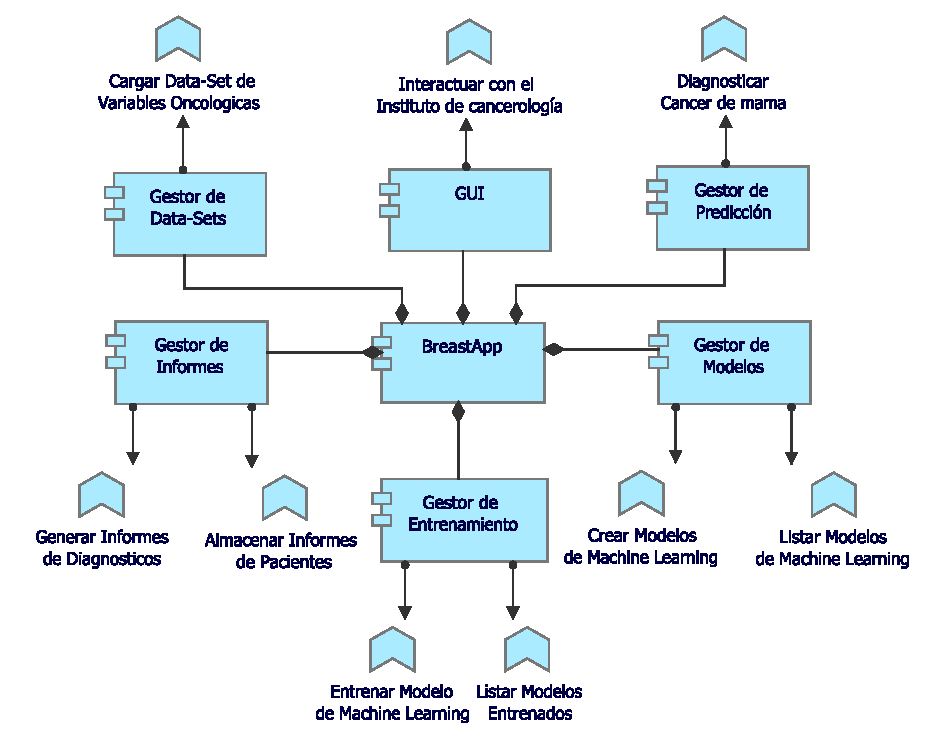
\includegraphics[width=1\linewidth]{ARQUITECTURA/imgs/CapaAplicacion/1_PvComportamientoApp}
	\caption{Punto de Vista del Comportamiento de la  Aplicación}
	\label{PvComportamientoApp}
\end{figure}

\begin{enumerate}[label=\textbf{\arabic*})]
	
\item  \textbf{BreastApp:} El componente de BreastApp es el framework  de la aplicación. En este componente se agregan los componentes correspondientes para el diagnóstico de cáncer de mama y se realiza la carga de modelos, carga de Data-Sets, entrenamiento de modelos  y generación de informes  sobre el cáncer de mama.

\item  \textbf{GUI:} Este componente esta agregado al componente principal de BreastApp. Este componente hace referencia a la interfaz gráfica de usuario por la cual los investigadores y unidades funcionales del Instituto  de Cancerología acceden a la aplicación, para llevar el análisis según diagnostico de cáncer de mama generado por la aplicación.Este componente cumple con la siguientes funciones:

	
\begin{itemize}
	\item  \textbf{\textit{Interactuar con el Instituto de Cancerologia:}} Hace referencia a las acciones y herramientas que contiene el Front-End de la aplicacion BreastApp las cuales pueden ser usadas po los investigadores de la Subdirección de Investigaciones, otras Subdirecciones y demás unidades funcionales del Instituto de Cancerología 
\end{itemize}
	
\item  \textbf{Gestor de Data-Sets:} Este componente esta agregado al componente principal de BreastApp. En este componente se maneja el proceso de carga  y gestión de Data-Sets para ser almacenados en el sistema.Este componente cumple con la siguientes funciones:
	
	\begin{itemize}
		\item  \textbf{\textit{Cargar Data-Set de Variables Oncológicas :}} Hace referencia a la carga del Data-Set para entrenamiento de los Modelos en Machine Learning y el Data-Set que contiene las variables Oncológicas de los pacientes a los cuales se les quiere detectar el padecimiento de cáncer de mama.
	\end{itemize}

\item  \textbf{Gestor de Entrenamiento:} Este componente esta agregado al componente principal de BreastApp. En este componente se maneja el proceso de entrenamientos de los modelos de Machine Learning haciendo uso de los Data-Sets  que estén almacenados en el sistema.Este componente cumple con la siguientes funciones:

	\begin{itemize}
		\item  \textbf{\textit{Entrenar Modelos de Machine Learning :}} Esta función realiza la mejora incremental para la predicción con Base en el Data-Set que contiene variables con resultados ya definidos de pacientes a los que ya se les detecto si el cáncer de mama era maligno o Benigno.
		
		\item  \textbf{\textit{Listar Modelo Entrenados:}} Esta función realiza una lista de los modelos a  los cuales ya se les realizo una mejora incremental de predicción para no repetir el proceso de entrenamiento cada vez que se requiere un diagnostico de cáncer de mama de diversos pacientes.
	\end{itemize}

\newpage
\item  \textbf{Gestor de Predicción:} Este componente esta agregado al componente principal de BreastApp. En este componente se maneja el proceso de diagnosticar el padecimiento de cáncer de mama. Este componente cumple con la siguiente función:
	\begin{itemize}
		\item  \textbf{\textit{Diagnosticar Cáncer de mama:}} Esta función realiza el diagnostico de cáncer de mama con base al entrenamiento anteriormente realizado , las variables de nuevos pacientes a los que se requiere realizar el análisis ontológico y las diversas técnicas de predicción y decisión de Machine Learning. 
	\end{itemize}

\item  \textbf{Gestor de Informes:} Este componente esta agregado al componente principal de BreastApp. En este componente se maneja el proceso generar informes con detalles del diagnóstico.Este componente cumple con la siguientes funciones:

\begin{itemize}
	\item  \textbf{\textit{Generar Informes de Diagnósticos:}} Esta función genera los informes tipo reporte con base a los resultados arrojados por los diferentes Modelos en Machine Learning, en donde se da un resultado definitivo acerca del  padecimiento de Cáncer de mama.
	
	\item  \textbf{\textit{Almacenar Informes de Pacientes:}} Esta función almacena los diferentes informes determinados a los pacientes a los que se quiere determinar el padecimiento de cáncer de mama.
\end{itemize}

\item  \textbf{Gestor de Modelos:} Este componente esta agregado al componente principal de BreastApp. En este componente se maneja el proceso implementación de  modelos de Machine Learning.Este componente cumple con la siguientes funciones:

\begin{itemize}
	\item  \textbf{\textit{Crear Modelos de Machine Learning:}} Esta función asocia los Data-Sets a los modelos de Machine Learning con los que realiza el respectivo diagnostico.
	
	\item  \textbf{\textit{Listar Modelos de Machine Learning:}} Esta función permite obtener los modelos de Machine Learning que utiliza el aplicativo de BreastApp.
\end{itemize}	
		
\end{enumerate}

%-------------Punto de Vista de Cooperación de Aplicación----------%
\newpage
\section{Punto de Vista de Cooperación de Aplicación}
El Punto de Vista de cooperación de la aplicación describe las relaciones entre los componentes de las aplicaciones en términos de los flujos de información entre ellos o en términos de los servicios que ofrecen y utilizan.\cite{BolanosCastro2019}.

En la Figura \ref{PvCooperacionApp} se plantea el Caso para el Punto de Vista de cooperación de la aplicación con cada uno de los elementos que interactúan entre sí. 

\begin{figure}[h!]
	\centering
	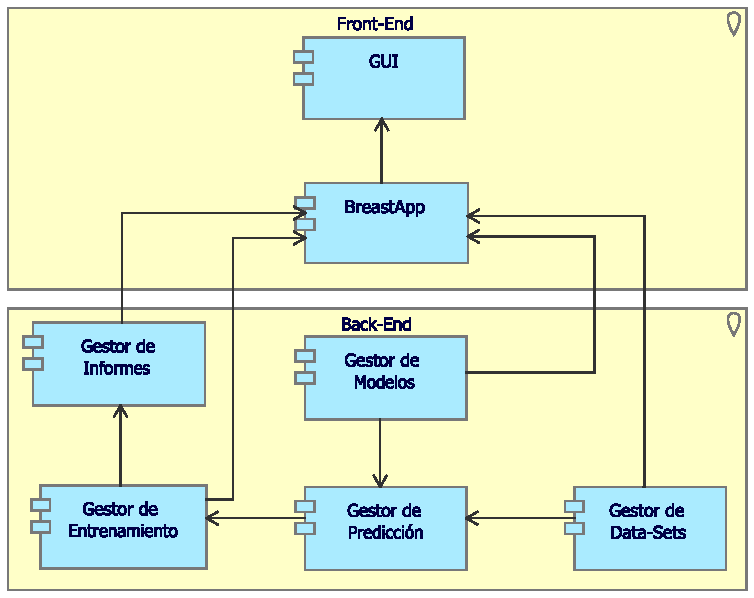
\includegraphics[width=1\linewidth]{ARQUITECTURA/imgs/CapaAplicacion/2_PvCooperacionApp}
	\caption{Punto de Vista de Cooperación de la Aplicación}
	\label{PvCooperacionApp}
\end{figure}

\begin{enumerate}[label=\textbf{\arabic*})]

\item  \textbf{BreastApp:} El componente de BreastApp es el framework  de la aplicación. En este se componente agregan los componentes correspondientes para el diagnóstico de cáncer de mama y se realiza la carga de modelos, carga de Data-Sets, entrenamiento de modelos  y generación de informes  sobre el cáncer de mama.
\item  \textbf{GUI:} Este componente esta agregado al componente principal de BreastApp. Este componente hace referencia a la interfaz gráfica de usuario por la cual los investigadores y unidades funcionales del Instituto  de Cancerología acceden a la aplicación, para llevar el análisis según el diagnostico de cáncer de mama generado por la aplicación.

\item  \textbf{Gestor de Modelos:} Este componente es usado por el componente principal de BreastApp y el componente Gestor de entrenamiento. En este componente se maneja el proceso de crear modelos.

\item  \textbf{Gestor de Predicción:} Este componente es usado por el componente de Gestor de Data-Sets y el componente Gestor de Modelos.En este componente se maneja el proceso de diagnosticar padecimiento de cáncer de mama.

\item  \textbf{Gestor de Data-Sets:} Este componente es usado por el componente principal de BreastApp y el componente Gestor de Predicción . En este componente se maneja el proceso de carga  y gestión de Data-Sets para ser almacenados en el sistema.

\item  \textbf{Gestor de Entrenamiento:} Este componente es usado por el componente principal de BreastApp y  el componente de Gestor de Predicción. En este componente se maneja el proceso de entrenamientos de los modelos de Machine Learning haciendo uso de los Data-Sets  que estén almacenados en el sistema.

\item  \textbf{Gestor de Informes:} Este componente es usado por el componente principal de BreastApp. En este componente se maneja el proceso Generar informes con detalles del diagnóstico.

\end{enumerate}


%-------------Punto de Vista de Estructura de Aplicación----------%
\newpage
\section{Punto de Vista de la Estructura de la Aplicación}
El Punto de Vista de estructura de la aplicación describe la estructura principal de aplicaciones o componentes y los datos asociados.\cite{BolanosCastro2019}.

En la Figura \ref{PvEstructuraApp} se plantea el Caso para el Punto de Vista de la estructura de la aplicación con cada uno de los elementos que interactúan entre sí. 

\begin{figure}[h!]
	\centering
	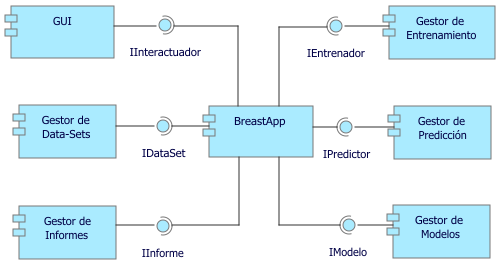
\includegraphics[width=1\linewidth]{ARQUITECTURA/imgs/CapaAplicacion/3_PvEstructuraApp}
	\caption{Punto de Vista de la Estructura  de la Aplicación}
	\label{PvEstructuraApp}
\end{figure}

\begin{enumerate}[label=\textbf{\arabic*})]
	
	\item  \textbf{BreastApp:} El componente de BreastApp es el framework  de la aplicación. En este se componente agregan los componentes correspondientes para el diagnóstico de cáncer de mama y se realiza la carga de modelos, carga de Data-Sets, entrenamiento de modelos  y generación de informes  sobre el cáncer de mama.
	\item  \textbf{GUI:} Este componente esta agregado al componente principal de BreastApp. Este componente hace referencia a la interfaz gráfica de usuario por la cual los investigadores y unidades funcionales del Instituto  de Cancerología acceden a la aplicación, para llevar el análisis según diagnostico de cáncer de mama generado por la aplicación, a través de la interfaz \textit{IInteractuador}.
	
	\item  \textbf{Gestor de Data-Sets:}Este componente ofrece un servicio a través de la interfaz \textit{IDataSet} al componente principal de BreastApp. En este componente se maneja el proceso de carga  y gestión de Data-Sets para ser almacenados en el sistema.
		
	\item  \textbf{Gestor de Informes:}Este componente ofrece un servicio a través de la interfaz \textit{IInforme} al componente principal de BreastApp. Este componente es usado por el componente principal de BreastApp. En este componente se maneja el proceso Generar informes con detalles del diagnóstico de cada paciente.
	
		
	\item  \textbf{Gestor de Entrenamiento:}Este componente ofrece un servicio a través de la interfaz \textit{IEntrenador} al componente principal de BreastApp. En este componente se maneja el proceso de entrenamientos de los modelos de Machine Learning haciendo uso de los Data-Sets  que estén almacenados en el sistema.
	
	\item  \textbf{Gestor de Predicción:}Este componente ofrece un servicio a través de la interfaz \textit{IPredictor} al componente principal de BreastApp. En este componente se maneja el proceso de diagnosticar padecimiento de cáncer de mama.
	
	\item  \textbf{Gestor de Modelos:} Este componente ofrece un servicio a través de la interfaz \textit{IModelo} al componente principal de BreastApp.En este componente se maneja el proceso de crear modelos.
\end{enumerate}

%-------------Punto de Vista de Uso de Aplicación----------%
\newpage
\section{Punto de Vista del Uso de la Aplicación}
El Punto de Vista del uso de la aplicación describe el diseño de una aplicación mediante la identificación de los servicios necesarios por los procesos de negocio y otras aplicaciones, o en el diseño de procesos de negocio mediante la descripción de los servicios que están disponibles \cite{BolanosCastro2019}.

En la Figura \ref{PvusoApp} se plantea el Caso para el Punto de Vista del uso de la aplicación con cada uno de los elementos que interactúan entre sí. 

\begin{figure}[h!]
	\centering
	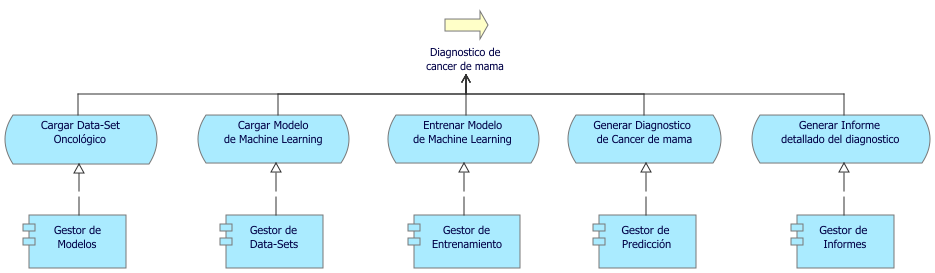
\includegraphics[width=1\linewidth]{ARQUITECTURA/imgs/CapaAplicacion/4_PvUsoApp}
	\caption{Punto de Vista del uso de la Aplicación}
	\label{PvusoApp}
\end{figure}

\begin{enumerate}[label=\textbf{\arabic*})]
	
	\item  \textbf{Diagnóstico de cáncer de mama:} Este proceso consiste en el diagnóstico de padecimiento de cáncer de mama. Es logrado mediante cinco servicios: \textit{Cargar modelo, Cargar Data-Set, Entrenar Modelo, Generar diagnóstico y Generar informe detallado del diagnóstico.} 
	
	\item  \textbf{Cargar Data-Set Oncológico:} Este servicio de la aplicación recibe los Data-Set con las variables oncológicas en formato .csv,  los valida  y los almacena en el sistema. Este servicio es realizado por el componente \textit{Gestor de Data-Sets}.
	
	\item  \textbf{Cargar Modelo de Machine Learning:} Este servicio de la aplicación es el encargado de crear modelos de Machine Learning. Este servicio es realizado por el componente \textit{Gestor de Modelos}.
	
	\item  \textbf{Generar Diagnostico de cáncer de mama:} Este servicio de aplicación recibe los datos de un paciente en particular  y realiza el diagnóstico. El servicio responde sí según los datos tiene un diagnóstico Benigno y Maligno. Este servicio es realizado por el componente \textit{Gestor de Predicción}.
	
	\item  \textbf{Generar Informe Detallado del Diagnostico:} Este servicio genera un informe detallado en formato .pdf con la información respectiva de las predicciones y gráficos de cada cada modelo.Este servicio es realizado por el componente \textit{Gestor de Informes}.
	
	

\end{enumerate}